% options:
% thesis=B bachelor's thesis
% thesis=M master's thesis
% czech thesis in Czech language
% slovak thesis in Slovak language
% english thesis in English language
% hidelinks remove colour boxes around hyperlinks

\documentclass[thesis=B,czech]{FITthesis}[2012/06/26]

\usepackage[utf8]{inputenc} % LaTeX source encoded as UTF-8

\usepackage{graphicx} %graphics files inclusion
% \usepackage{amsmath} %advanced maths
% \usepackage{amssymb} %additional math symbols

\usepackage{dirtree} %directory tree visualisation


\usepackage{listings}
\lstset{frame=lrbt,xleftmargin=\fboxsep,xrightmargin=-\fboxsep, showstringspaces=false}

% % list of acronyms
% \usepackage[acronym,nonumberlist,toc,numberedsection=autolabel]{glossaries}
% \iflanguage{czech}{\renewcommand*{\acronymname}{Seznam pou{\v z}it{\' y}ch zkratek}}{}
% \makeglossaries

\newcommand{\tg}{\mathop{\mathrm{tg}}} %cesky tangens
\newcommand{\cotg}{\mathop{\mathrm{cotg}}} %cesky cotangens

% % % % % % % % % % % % % % % % % % % % % % % % % % % % % % 
% ODTUD DAL VSE ZMENTE
% % % % % % % % % % % % % % % % % % % % % % % % % % % % % % 

\department{Katedra Softwarového inženýrství}
\title{Webový server pro poskytování dynamicky generovaných objektů ve formátech RDF}
\authorGN{Jan} %(křestní) jméno (jména) autora
\authorFN{Řasa} %příjmení autora
\authorWithDegrees{Jan Řasa} %jméno autora včetně současných akademických titulů
\supervisor{RNDr. Jakub Klímek, Ph.D.}
\acknowledgements{Díky všem}
\abstractCS{Řada objektů na webu dat tvoří natolik velkou skupinu (až nekonečnou), že je není možné všechny 
perzistentně uložit a publikovat. Je nutné nabídnout server, který na základě požadavku klienta na daný 
objekt příslušná data dynamicky vygeneruje a odešle klientovi.
Tato práce se zabývá
Cílem této práce je analýza již existujících řešení, návrh a implementace daného serveru. Server bude 
umožňovat uživateli definovat RDF (Resource Description Framework) objekty pro dynamické 
generování v několika formátech. Součástí této práce je také návrh vhodných formátů pro tyto definice.
Návrh bude zohledňovat již zaběhlé technologie z oboru Linked data, jako je například dotazovací 
jazyk SPARQL (Protocol and RDF Query Language). Server bude implementován v jazyce Java.}
\abstractEN{Sem doplňte ekvivalent abstraktu Vaší práce v~angličtině.}
\placeForDeclarationOfAuthenticity{V~Praze}
\declarationOfAuthenticityOption{4} %volba Prohlášení (číslo 1-6)
\keywordsCS{sémantický web, linked data, RDF, dynamické generování, SPARQL, java, webový server}
\keywordsEN{Nahraďte seznamem klíčových slov v angličtině oddělených čárkou.}

\begin{document}

% \newacronym{CVUT}{{\v C}VUT}{{\v C}esk{\' e} vysok{\' e} u{\v c}en{\' i} technick{\' e} v Praze}
% \newacronym{FIT}{FIT}{Fakulta informa{\v c}n{\' i}ch technologi{\' i}}

\begin{introduction}
\paragraph{}
Při publikování dat na webu dat je vždy důležité zamyslet se nad tím, jak a kde budou tyto data uložena.
Způsobů je mnoho. Mezi ty nejzákladnější patří ukládání dat do různých databázových systémů, nebo pouze přímo na určené místo na disku.
Oba zmíněné způsoby a jim podobné mají ovšem jeden zásadní problém, a tím je kapacita uložiště.

Pro uložení většiny informací, se kterými se lze setkat na webu, jako jsou obrázky, zprávy, informace o počasí a mnoho dalších, se tato skutečnot nemusí příliš řešit.
Kapacita uložiští nám pro tyto informace stačí. Nicméně existuje řada informací(dále také objektů), které tvoří natolik velkou skupinu (až nekonečnou),
že je není možné všechny perzistentně uložit a publikovat.

Dobrým příkladem jsou například časová data - konkrétní čas či časový interval. V kontextu Linked Data \cite{linked_data} se často odkazuje na časový objekt.
Ať už se jedná například o časy příjezdů autobusů nebo o datum nějaké události, vždy je potřeba mít daný časový objekt nějakým způsobem uložen.

Existují ale kapacity na uložení každého takového objektu? Časových objektů je přeci nekonečně mnoho. Mohou odkazovat jak do minulosti, tak do budoucnosti.
A není potřeba se omezovat pouze na časové objekty. Jako další příklad může být informace o vztahu mezi lidmi, respektive mezi kterýmikoliv subjekty.
Tyto informace taktéž vyžadují ohromné kapacity uložiští.

Všechny tyto objekty ale spojuje fakt, že mají vždy stejnou strukturu a jen část informací se mění(například jen sekunda, nebo jméno člověka).
A to je ideální příležitost pro to, aby se ukládání těchto objektů zaměnilo za dynamické generování. Pro vygenerování objektu stačí vždy použít stejnou strukturu
a jen dosadit potřebné informace tak, aby vznikl požadovaný objekt.

\end{introduction}

\chapter{Cíl práce}
Cílem této práce je navrhnout, implementovat a otestovat webový server pro poskytování dynamicky generovaných objektů v RDF formátech.
Server bude splňovat následující požadavky:

 \begin{itemize}
  \item Server bude umožňovat administrátorovi založit nový typ objektů včetně jejich atributů a umožní nakonfigurovat URL, pod kterými budou objekty dostupné. 
  \item Typy objektů bude možné založit přes konfigurační soubor. 
  \item Klient bude moci přístupem na dané URL získat data o příslušném objektu. 
  \item Data o objektech budou klientům dostupná v RDF serializacích (RDF/XML, Turtle, N-Triples, JSON-LD) a jako webová stránka.
  \item Server bude využívat mechanismu Content Negotiation pro určení formátu výstupu požadavku klienta. 
  \item Server bude implementován v jazyce Java.
 \end{itemize}
\chapter{Analýza}

\section{Účel aplikace}
Webový server bude poskytovat uživatelům funkci pro dynamické generování objektů ve formátech RDF.
Uživatel si bude moci nadefinovat vlastní typy objektů pomocí šablony včetně URL, na které budou dané objekty přístupné.
Objekty budou generovány za použití informací, které bude obsahovat URL adresa při požadavku na daný objekt.

Tento způsob generování objektů ve velké míře šetří především finanční zdroje za pořizování nových uložišť. Pro velké množství stejných objektů (až nekonečně mnoho)
stačí vytvořit pouze jednu definici (šablonu) objektu, která se dle specifikovaných pravidel vyplní informacemi z URL adresy a uživateli se zobrazí jako 
požadovaný objekt.

Další výhodou je z hlediska jednotné definice objektů i možnost lehce upravit strukturu konkrétních definic na jednom místě.
Na konkrétní definici objektu může být odkazováno s různými parametry z mnoha jiných objektů a jedinou změnou v definici lze ovlivnit informace i v těchto objektech.
Měnit již dříve vytvořené a uložené konkrétní objekty v takovém počtu by bylo téměř nereálné.

Účelem serveru je také chování, které co nejméně omezuje možné klienty \footnote{Zde se klientem rozumí především aplikace které by k objektům přistupovaly.}.
Server využívá principu Content Negotiation \cite{content_negotiation} a podporuje nejpoužívanější typy RDF serializací, včetně možnosti zobrazit informace 
o objektu v HTML podobě při zobrazení prohlížečem.


\section{Existující řešení}
Pro funkce, které má tento server splňovat, neexistuje v současnosti žádné jiné řešení. Minimálně není možné dohledat 
  žádné veřejné řešení, ani informace o nějakém soukromém řešení, které by sloužilo například pro soukromá data v rámci nějaké společnosti. 
  Nicméně existuje velmi populární řešení jednoho typu objektu - časových intervalů, tzv. British Time Intervals, které je hojně používané,
  převážně pak také v rámci dat, které poskytuje britská vláda.
  
\subsection{British Time Intervals}
Pro popis těchto objektů je asi nejlepší odkázat se na konkrétní definici na webové stránce, ze které jsou tyto intervaly dostupné.\cite{british_ti}
\begin{quote}
 Linked data for every time interval and instant into the past and future, from years down to seconds.
 This is an infinite set of linked data. It includes government years and properly handles the transition to the Gregorian calendar within the UK.
\end{quote}
 Zde je vhodné všimnout si hlavně slov \textit{infinite set}, což přesně charakterizuje typy objektů, kterými se tato práce zabývá.

 \subsubsection{Struktura URI} Pro přístup k jednotlivým generovaným objektům slouží URL adresa, která má vždy předepsanou strukturu. Informace, které jsou dostupné
k tomuto datasetu, obsahují popis těchto struktur a jsou veřejně dostupné na stránkách společnosti Epimorphics \cite{ti_structure}. Takovou URL adresou může být například 
\textit{http://reference.data.gov.uk/doc/government-year/\{year1\}-\{year2\}}, kde po dosazení let míto \textit{year1} a \textit{year2} a přístupem na danou adresu získáme požadovaný 
objekt časového intervalu.

\subsubsection{Generování objektu} Takový objekt je tedy dynamicky vygenerován s použitím parametrů z URL adresy. Konkrétní popis toho, jak jsou tyto objekty interně generovány 
není veřejný, ale je velmi pravděpodobné, že je použit minimálně jeden z následujících způsobů:
\begin{itemize}
  \item Předem připravená RDF šablona (v libovolném formátu - Turtle, RDF/XML, N-TRIPLES \ldots) s placeholdery, do kterých se dosadí parametry z URL adresy.
  \item SPARQL \cite{sparql_w3c}\cite{sparql_bob} dotaz s placeholdery.
 \end{itemize}

 

\section{Požadavky}

\subsection{Funkční požadavky}
 \begin{itemize}
  \item přístup k administraci objektů přes více rozhraní
  \item podpora více formátů pro definice a zobrazení objektů
  \item zobrazení existujících definic objektů
  \item administrace definic objektů  
  \item konfigurace objektů bude možná několika způsoby
  \item vygenerování a zobrazení konkrétních objektů
 \end{itemize}
 
 \subsubsection{Přístup k administraci objektů přes více rozhraní}
 Administrátori bude umožněn přístup k definicím objektů dvěma způsoby:
 \begin{itemize}
    \item přes webové rozhraní
    \item přes API
 \end{itemize}
 Oba tyto způsoby budou poskytovat stejnou funkcionalitu. Webovým rozhraním se myslí jednoduchá aplikace pro administraci objektů z webového prohlížeče.
 API bude sloužit k administraci z jiných potenciálních aplikací.
 
 \subsubsection{Podpora více formátů pro definice a zobrazení objektů}
 Server bude podporovat následující formáty pro definice objektů přes API:
 \begin{itemize}
    \item JSON formát \cite{JSON}
    \item RDF serializace TURTLE \cite{turtle}
 \end{itemize}
 Konkrétní vygenerované objekty budou klientům dostupné v těchto RDF serializacích:
 \begin{itemize}
    \item RDF/XML \cite{rdf_xml}
    \item JSON-LD \cite{json_ld}
    \item N-TRIPLES \cite{n_triples}
    \item TURTLE 
 \end{itemize}
 Každá definice objektů bude také umožňovat definovat HTML formát objektu pro zobrazení v prohlížeči.
 
 \subsubsection{Zobrazení existujících definic objektů}
  Ve webové aplikaci budou zobrazeny všechny aktuální definice objektů v tabulce s možností konkrétní definici upravit (tedy také zobrazit definici konkrétního objektu)
  nebo smazat přes tlačítka vedle každé definice.
  
  Přes API bude možné získat definice objektů ve dvou formátech:
  \begin{itemize}
    \item RDF serializace
    \item JSON formát
 \end{itemize}
  Konkrétní formát bude určen principem Content Negotiation. Získat půjde seznam všech definic a také konkrétní definice.
 
 \subsubsection{Administrace definic objektů}
  Administrátorovi bude umožněno přidávat nové definice, měnit a mazat již vytvořené definice. Tyto akce budou umožněny jak z webové aplikace, tak i přes API.
  Dále bude moci administrátor definovat objekt konfiguračním souborem v RDF serializaci TURTLE.
  
  
  \subsubsection{Konfigurace objektů bude možná několika způsoby}  
  \label{sec:object_types}
  Koknfigurací objektů se zde myslí možné způsoby jak a z čeho se bude generovat výsledný RDF objekt. Server bude podporovat
  následující způsoby:
  \begin{itemize}
    \item generování ze SPARQL šablony - CONSTRUCT dotaz \cite{sparql_construct}
      \subitem Vstupem bude SPARQL šablona CONSTRUCT dotazu s placeholdery \footnote{Placeholder: část šablony, která jasně identifikuje místo, 
      kam se dosadí parametry z URL adresy.}, za které se dosadí při požadavku na objekt hodnoty z URL adresy
      a provede se příkaz který vygeneruje objekt.
      
     \item generování ze SPARQL šablony - vzdálený CONSTRUCT nebo DESCRIBE dotaz \cite{sparql_describe}
      \subitem Vstupem bude SPARQL šablona jako v prvním případě. Navíc bude možné provést DESCRIBE dotaz. Rozdíl oproti prvnímu případu je v tom, že se 
      dotaz přepošle na zvolenou adresu SPARQL Endpointu \cite{sparql_endpoint}, zde se provede a klientovy je pak vrácen daný objekt.
      
    \item generování z RDF šablony
     \subitem Vstupem bude RDF šablona podporovaných serializací s placeholdery, za které se dosadí při požadavku na objekt hodnoty z URL adresy. 
     
     \item Proxy objekt
      \subitem Server bude umožňovat roli prostředníka při generování objektů. Požadavek na objekt se přepošle na jiný server a výsledek se přeloží
      klientovi dle požadované serializace. Tento způsob umožňuje generování objektů přes jiné aplikace.
 \end{itemize}
 
 
  
  \subsubsection{Vygenerování a zobrazení konkrétních objektů}  
  Klient bude moci přístupem na konkrétní URL adresu získat data o příslušném objektu. Typ RDF serializace nebo zobrazení HTML stránky se určí přes 
  Content Negotiation.

\subsection{Nefunkční požadavky}
\begin{itemize}
    \item server bude implementován v jazyce Java
    \item celá aplikace bude uložena ve WAR souboru pro zjednodušené nasazení
 \end{itemize}
 
 \chapter{Návrh}
 
 \section{Použité technologie}
 
 \subsection{Resource Description Framework (RDF)}
 Resource Description Framework je rodina specifikací, která se používá jako metoda pro modelování informací - objektů.
 Jedná se o model metadat, které popisují nějaké zdroje.
 
 Příkladem může být obyčejná webová stránka obsahující nějaké informace. Webové stránky se zaměřují především na uživatele.
 Důležité je, aby se uživateli stránky líbily a dbá se tedy hodně na design. Pokud jsou stránky přehledné, pak člověk nemívá problémy pochopit
 dané informace. Nicméně stroj (počítač, program) tyto informace sice zobrazí uživateli, ale samotné informace si interpretovat nedokáže.
 
 RDF model popisuje tedy způsoby, jakými docílit toho, že poskytované informace budou čitelné i pro stroje.
 
 Základní kostrou RDF modelu dat jsou takzvané $trojice$. Tyto trojice se skládají ze subjektu, predikátu a objektu.
 Trojice se může volně přeložit i do podoby, kde subjekt má nějakou vlastnost (predikát) s konkrétní hodnotou (objekt). Tedy všechny trojice, které mají
 stejný subjekt tento subjekt definují.
 
 Každý subjekt je identifikován nejčastěji přes URI. Bavíme-li se o datech na webu, tak zde může být URI klasická URL adresa, jak ji známe
 z běžného používání. Co se týče objektu (hodnoty), tak se může jednat o literál (řetězec, číslo apod.), ale hodnotou může být zase URI nějakého dalšího objektu.
 Dokonce i predikát může být objektem s vlastním URI. Tím, že se objekt skládá z dalších objektů, které jsou jednoznačně identifikovány pomocí URI, získáváme velkou výhodu
 tohoto modelu. Ve výsledku vzniká graf popisující tyto trojice, což je i pro stoje čitelná struktura.
 
 Samotné RDF popisuje pouze model. Pro uložení tohoto modelu je zapotřebí informace nějakým způsobem serializovat. Pro uložení RDF objektů se 
 používají nejčastěji tyto RDF serializace:
 \begin{itemize}
  \item RDF/XML
  \item Turtle
  \item N-Triples
  \item JSON-LD
 \end{itemize}
 
 Pro ukázku je zde příklad ve formátu Turtle, který je převzat z W3C specifikace \cite{turtle_example}.
 \begin{lstlisting}[language=C, basicstyle=\small]
@base <http://example.org/> .
@prefix rdf: <http://www.w3.org/1999/02/22-rdf-syntax-ns#> .
@prefix rdfs: <http://www.w3.org/2000/01/rdf-schema#> .
@prefix foaf: <http://xmlns.com/foaf/0.1/> .
@prefix rel: <http://www.perceive.net/schemas/relationship/> .

<#green-goblin>
    rel:enemyOf <#spiderman> ;
    a foaf:Person ;  # in the context of the Marvel universe
    foaf:name "Green Goblin" .

<#spiderman>
    rel:enemyOf <#green-goblin> ;
    a foaf:Person ;
    foaf:name "Spiderman".
\end{lstlisting}
<$\#green-goblin$> je zde subjekt identifikovaný URI (http://example.org/\#green-goblin),
$rel$:$enemyOf$ je predikát - v tomto případě zase objekt identifikovaný URI (http://www.perceive.net/schemas/relationship/enemyOf) a 
 <$\#spiderman$> je objekt - zase identifikován URI.
 Tento model dohromady poskytuje informaci, že objekt na dané URI je nepřítelem Spidermana. $a foaf$:$Person$ znamená, že
 se jedná o objekt Person a $foaf:name "Green Goblin"$ zase to, že jeho jméno je Green Goblin. Tímto je tedy definován objekt $<\#green-goblin>$ a podobně tomu je u 
 objektu <$\#spiderman$>.
 
 \subsection{Linked Data}
  Linked data, jak už název napovdá, popisuje metodu propojování informací na webu dat mezi sebou.  
  Tim Berners-Lee, zakaldatel WWW,  popisuje Linked Data výstižně takto: 
  \uv{\textit{Semantic Web isn't just about putting data on the web. It is about making links, so that a person or machine can explore the web of data. 
  With linked data, when you have some of it, you can find other, related, data.}} \cite{TimBL_LD}
  
  Aby se publikovaná data mohly využívat v co největší míře, nestačí je pouze zpřístupnit na webu dat. Největší užitek přináší linkování těchto dat dohromady.
  Stejně, jak je tomu u HTML dokumentů, slouží pro linkování v rámci RDF URI, které jasně identifikují objekty. Nad takto prolinkovanými daty se poté dají
  najít různé vztahy, které by bez prolinkování nebylo monžé nalézt.
  
  Linked Data staví na těchto čtyřech základních principech:
  \begin{itemize}
   \item Pro názvy a identifikaci objektů se používá URI
   \item Aby byly data přístupné, používají se HTTP URI
   \item Při přístupu na konkrétní URI lze získat informace dle standardů RDF, SPARQL, \ldots
   \item Na ostatní data se odkazuje také přes HTTP URI
  \end{itemize}
  
  Při zohlednění všech těchto principů lze získat maximálně propojené informace a jak už bylo u RDF zmíněno, ve výsledku vznikne ohromný graf vzájemně
  propojených informací, ve kterém je možné následně najít cenné informace i o objektech, které na první pohled nemusí mít mezi sebou nic společného.

  
  \subsection{Java}
   Při vývoji je použit programovací jazyk Java. Použití javy vychází už z požadavků ze zadání. Hlavní důvody, proč je zde java vhodná a proč byla
   i jedním z požadavků jsou následující:
   \begin{itemize}
    \item Rozšířenost javy ve světě Linked Data
    \item Snadná integrace kvalitních knihoven pro práci s RDF
    \item Jednoduše nasaditelná aplikace přes webový archiv (war soubor)
    \item Výkon
   \end{itemize}
   Rozšířenost javy ve světě Linked Data je opravdu velká. Důvodem, proč je tento fakt zmíněn ve výhodách, je možnost případné snadné integrace dalších systémů
   pro vývojáře z tohoto oboru. Důležitým důvodem je zmíněný výkon aplikace. Na ten mají vliv jak knihovny pro práci s RDF, tak ale i samotný typ aplikace.
   Server si může uchovávat předzpracované šablony, patterny regulárních výrazů a další informace přímo v paměti, tudíž klient ve výsledku dostane výsledek rychleji,
   než by tomu bylo při použití například PHP nebo podobných jazyků.
   
   \subsection{Apache Jena}
   Pro práci s RDF daty byla zvolena knihovna Apache Jena. Tato knihovna podporuje práci přímo s RDF serializacemi a díky procesoru ARQ také práci se SPARQL
   dotazy. Další možností pro použití byla knihovna Sesame. Knihovny si jsou velice podobné. Obě mají dobrou dokumentaci i velmi dobře zpracované 
   ukázky, jak lze knihovny využívat. Rozhodujícím faktorem při výběru byl výkon.
   
   Při výkonostním srovnání byl zohledněn publikovaný test \textit{The Berlin\\ SPARQL Benchmark} \cite{sparql_benchmark}.
   Jena a Sesame se dle něj výkonostně velmi liší. Sesame je několikanásobně rychlejší na dotazování, ale Jena naopak s velkým náskokem vede při načítání souborů
   v Turtle formátu.
   
   Výkonostně má vliv načítání definic objektů, které se uchovávají v turtle formátu. Jedná se o proces, který bude spuštěn při zapnutí aplikace a při
   případném novém načtení (reloadu) definic (v případě nahrání definice přímo do filesystému dle požadavku). Rychlost SPARQL dotazů tedy není v tomto
   případě tolik důležitá. Při požadavku klienta na vygenerování objektu už se s RDF definicí nijak nepracuje - není potřeba se nad definicemi dále dotazovat.
   U typů SPARQL Endpoint/Construct také nedocházi k dotazovaní se nad lokálně uloženými daty.
   
   \subsection{Další Java knihovny}
   \begin{itemize}
    \item Jersey, GSON - pro práci s definicemi objektů v rámci API
    \item Log4j - logovací systém
    \item Typesafe - konfigurace
    \item JUnit - testování
   \end{itemize}
   
   \subsection{Maven}
   Závislosti, sestavení a testování se provádí přes build manažer Maven. Maven byl vybrán jako standard pro většinu Java aplikací.
   Vývoj taktéž probíhal v IDE IntelliJ IDEA, které obsahuje velmi dobrou integraci tohoto systému.
   
   \subsection{AngularJS}
   Součástí celého systému je i webová aplikace pro správu definic objektů. Zde je použit framework AngularJS, který je snadno napojitelný
   na REST API serveru. 

   \newpage
   
 \section{Návrh architektury}
  Na diagramu \ref{parts} lze vidět, že je systém rozdělen do 2 částí. První částí je webová aplikace, která slouží pro ulehčení administrace definic objektů.
  Hlavní funkcionalita tohoto serveru ale není touto částí ovlivněna, na API se lze napojit i z jiných aplikací.
  Tato část je napsaná ve frameworku AngularJS která využívá serverové API.
  U této aplikace se dá mluvit o známé MVC\footnote{Model-View-Controller} architektuře, kde je ovšem Model (zde definice objektu)
  primárně součástí druhé části systému.
  
  Druhou částí je serverová část, dále také pod názvem \textit{Jádro systému}. Architektura této části je velice podobná MVC architektuře. O čistém MVC nelze 
  mluvit z toho důvodu, že je zde velká provázanost komponent a není až tak striktně oddělena zodpovědnost jednotlivých částí.
  
  \begin{figure}\centering
 	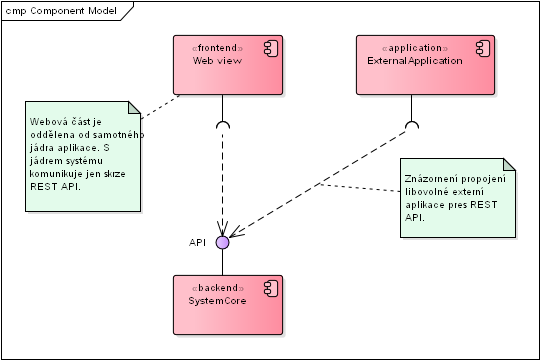
\includegraphics[width=1\textwidth]{parts}
 	\caption[Model tříd]{Dvě základní části systému (jádro systému a webová, nebo jakákoliv jiná aplikace napojená na API)}\label{parts}
 \end{figure}
  
  \subsection{Jádro systému}  
  Jádro systému se skládá ze čtyř hlavních komponent, které lze také vidět na obrázku \ref{packages_core}. Pro administraci definic objektů slouží komponenta API. Další komponentou je Model, který obsahuje
  třídy využívané všemi komponentami. O načítání, ukládání a přístup k definicím objektů se stará komponenta Container.
  Poslední základní komponentou je Publisher, který zpřístupňuje celý systém klientovi v podobě vygenerovaných objektů.
  
  
  \begin{figure}\centering
 	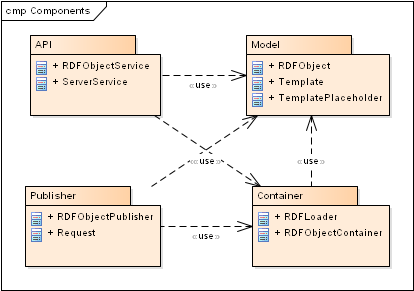
\includegraphics[width=0.8\textwidth]{packages_core}
 	\caption[Model komponent]{Základní čtyři komponenty jádra systému}\label{packages_core}
 \end{figure}
  
  \subsubsection{Komponenta API}
    Tato komponenta slouží pro administraci definic objektů. Jedná se o komponentu, ke které má přístup pouze administrátor systému. Obsahuje dvě třídy, které
    mají své metody vystavené pro napojení přes API.
    
    Tyto třídy jsou zobrazeny na obrázku \ref{api_class}. Třída RDFObjectService slouží k samotnému vytváření, úpravě a mazání definic. ServerService pak obsahuje
    metodu, která se dá taktéž volat přes API a slouží ke znovunačtení všech definic z nastaveného uložiště.
    \begin{figure}\centering
 	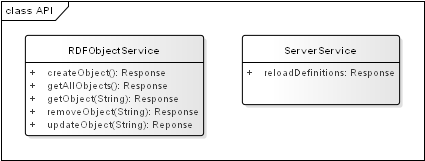
\includegraphics[width=0.8\textwidth]{api_class}
 	\caption[Model tříd]{Třídy reprezentují služby, které mají metody vystavené pro API}\label{api_class}
    \end{figure}
    
    \subsubsection{Komponenta Model}
    Tato komponenta obsahuje tři základní třídy, které jsou využívány zbytkem aplikace. Jedná se o třídy RDFObject, Template a TemplatePlaceholder, které jsou zobrazeny
    na obrázku \ref{model_class}.
    
     \begin{figure}\centering
 	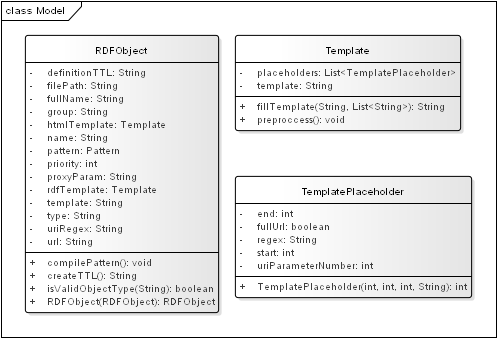
\includegraphics[width=\textwidth]{model_class}
 	\caption[Model tříd]{Třídy v komponentě Model. Pro přehled jsou uvedeny pouze nejdůležitější metody. Třídy jinak obsahují i další metody, převážně settery a gettery.}\label{model_class}
    \end{figure}
    
    RDFObject reprezentuje samotnou definici objektu. Obsahuje dva atributy typu Template. Prvním z nich je šablona definice (RDF serializace, nebo SPARQL dotaz) a
    druhou je HTML šablona sloužící pro zobrazení objektu v HTML formátu. Dále obsahuje metody jako jsou například validace a kompilace patternu
    regulárního výrazu pro pozdější identifikace definice dle požadavku klienta. Obsahuje také gettery a settery pro atributy, které ale nejsou
    na zmíněném diagramu vidět pro jejich primitivnost.
    
    Třídy Template a TemplatePlaceholder zastřešují celý šablonovací systém. Třída Template obsahuje dvě důležité metody pro přdzpracování šablony
    a následné vyplnění šablony při požadavku. Předzpracování šablony probíhá tak, že se v šabloně naleznou všechny placeholdery a uloží se do seznamu
    pro pozdější vyplnění. Předzpracování probíhá pouze jendou při nahrátí definic (při startu serveru nebo znovunačtení definic). Cílem takto
    předzpracované šablony je urychlení generování objktů tak, aby se pouze dosazovaly hodnoty a případně aplikovaly podporované regulární výrazy.
 
 \subsubsection{Komponenta Container}
 O správu nahraných definic se stará komponenta Container. Z obrázku \ref{container_class} je patrné, že obsahuje 2 třídy.
 
 Třída RDFLoader se stará
 o čtení jednotlivých definic z file systému, validaci a následnou transformaci definice v Turtle formátu do objektu RDFObject,
 který reprezentuje konkrétní definice.
 
 Třída RDFContainer slouží jako kontejner (malá databáze) všech nahraných objektů. Objekty si drží jak podle celého jména definice pro rychlý přístup
 k definicím pro API, tak i podle priorit, podle kterých dochází k vyhledávání definic při požadavku klienta.
 Kontejner se v aplikaci vyskytuje díky použití singleton patternu
 pouze jeden a je nejvytíženějším objektem v celé aplikaci, protože je využíván všemi komponentami.
 
 \begin{figure}\centering
 	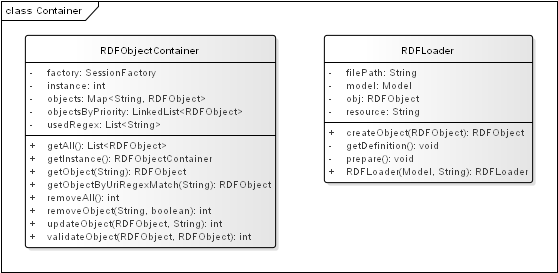
\includegraphics[width=\textwidth]{container_class}
 	\caption[Model tříd]{Komponenta container obsahuje třídy pro administraci objektů}\label{container_class}
    \end{figure}
    
    \subsubsection{Komponenta Publisher}
    Tato komponenta slouží k odbavování požadavků klienta na vygenerování objektu. Na obrázku \ref{publisher_class} lze vidět 2 třídy,
    které mají za úkol interakci s klientem.
    
    Třída RDFObjectPublisherService zpracovává prvotní požadavek klienta metodou $handleObjectRequest()$. V rámci systému je tato metoda definována
    pro všechny podporované serializace výstupu (HTML, RDF/XML, Turtle, JSON-LD a N-Triples). Při zavolání těchto metod je dále vytvořen 
    objekt třídy Request, kterému je předána zodpovědnost za vygenerování výsledného objektu. 
    
    \begin{figure}\centering
 	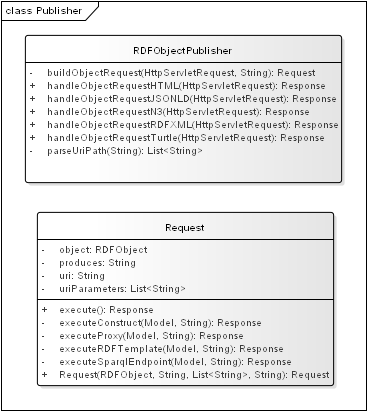
\includegraphics[width=0.8\textwidth]{publisher_class}
 	\caption[Model tříd]{Komponenta container obsahuje třídy pro administraci objektů}\label{publisher_class}
    \end{figure}
    
    
   \newpage
   
   
 
 \section{Identifikace objektů, URL}
 \label{sec:identifikace}
 V kontextu RDF se dají objekty identifikovat pouze jedním způsobem, a to URL adresou. V tomto případě ale URL zastává ještě jednu důležitou úlohu.
 Vzhledem k tomu, že je jediným spojením mezi objektem (a jeho definicí) a vnějším prostředím, tak musí nést i informace, ze kterých bude později vygenerován
 konkrétní objekt. Návrhu struktury URL byla proto věnována velká pozornost.
 
 \subsection{Struktura URL v.1}
 Prvotní návrh byl takový, že se URL rozdělí na následující 3 části:
 \begin{itemize}
  \item Hostname
   \subitem Touto částí se rozumí identifikace serveru a protokolu, například \textit{https://dynrdf.com}. Z pohledu objektu slouží jen jako část identifikátoru.

    \item Identifikace objektu - první část cesty za hostname
     \subitem Tato část slouží k identifikaci objektu. Jedná se o unikátní název pro každý objekt. Příkladem může být například objekt časového intervalu s URL začínající 
     \textit{https://dynrdf.com/time-interval}, kde \textit{time-interval} identifikuje tento objekt.
     
    \item Parametry objektu
     \subitem Zbývající část URL nese informace, které se dosadí do šablon jednotlivých definic objektů. Jednotlivé parametry jsou vždy odděleny lomítkem.
     Například pro objekt ročního intervalu by mohla URL vypadat následovně \textit{https://dynrdf.com/time-interval/2015/2016}, kde by zvolené roky znamenaly 
     parametry \textit{od} a \textit{do}.
 \end{itemize}
 Tento návrh by byl naprosto dostačujícím pro generování objektů všech podporovaných typů. Nicméně s sebou nese dva velké problémy.
 
 Prvním problémem je ten, že by musel být každý objekt identifikován IP adresou nebo doménou, kde tento server bude spuštěn. To by tedy znamenalo, že
 by tu nebyla možnost určit pro každý objekt extra URL v identifikátoru. Pokud by například funkce tohoto serveru chtěly využívat dvě různé společnosti, které
 by svoje objekty dále publikovali, tak by mohlo docházet k nekonzistenci odkazů na objekty. Jinými slovy se dá také zeptat na to, proč by nějaká společnost chtěla 
 publikovat data, kde jejich identifikace není spojena například s názvem společnosti. Vždy by v identifikaci figuroval tento server, který ale s původem dat nemá
 nic společného. Cílem tohoto systému je pouze generovat objekty a identifikaci a vlastnictví ponechat na autorovi daných definic objektů.
 
 Druhý problém, nebo spíše nepříjemnost nastavá v případě, že by se servery společností využívající tohoto dynamického generování chovali jako prostředníci 
 a požadavky na objekty přeposílaly na tento server. Pokud by každá definice měla vždy konkrétní unikátní identifikátor v URL adrese, pak by se pro každý takový objekt 
 muselo přidávat pravidlo ve webových serverech na přeposílání požadavku a případně i dál složitě parsovat URL z požadavku na primárním serveru na URL, která by byla 
 dle zmíněných specifikací.
 
 Pro lepší představu, jak může vypadat požadavek na konkrétní objekt přes prostředníka, třetí stranu, slouží obrázek \ref{request_flow_2}. Při požadavku
 přímo na tento server z klienta se proces na jiném serveru přeskočí. Ani jeden z těchto způsobů právě není bez nějakého výše zmíněného problému. 
 \begin{figure}\centering
 	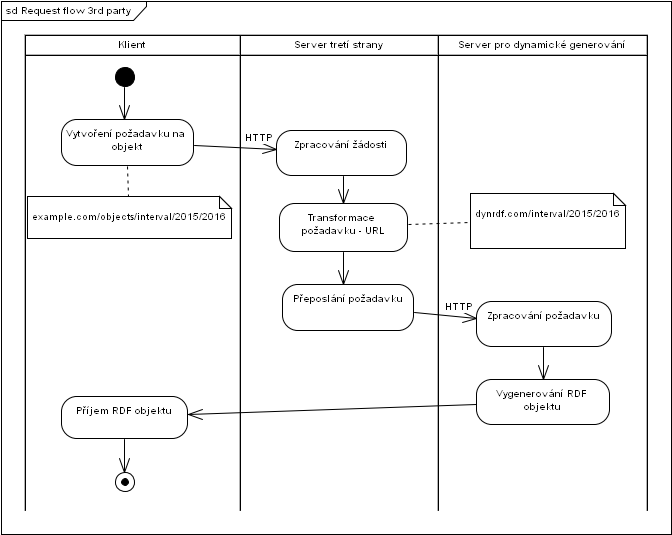
\includegraphics[width=1\textwidth]{request_flow_2}
 	\caption[Požadavek na objekt přes server třetí strany]{Požadavek na objekt přes server třetí strany. Prvotní návrh struktury URL adresy.}\label{request_flow_2}
 \end{figure}
 
 \subsection{Struktura URL v.2}
  Výše zmíněný návrh by znamenal téměř nepoužitelnost tohoto systému. Bylo proto nutné navrhnout jiné řešení. To se od původního návrhu liší na dvou místech, v předání
  informací o objektu a identifikací objektů.
  
  \subsubsection{Informace o objektu v GET parametru}
   Předání dat o objektu v GET parametru naprosto jednoduše řeší problém s parsováním URL adresy na serverech třetích stran. V případě, kdy na jiný server přijde požadavek
   na nějaký objekt, tak stačí v konfiguraci webových serverů nastavit pouze jedno pravidlo pro přeposlání požadavku pro všechny objekty.
  
  \subsubsection{Identifikace objektů, regulární výraz}
   Předání informací o objektu v GET parametru má ale za následek, že URL adresa už neobsahuje identifikátor objektu jako první část cesty. Objekt se dá identifikovat 
   pouze z informací v GET parametru, pro který účelově není stanovena žádná struktura.
   
   Strukturu URL adresy v GET parametru, která má identifikovat konkrétní objekt, zná pouze autor definice. Ideálním nástrojem, jak docílit mapování URL na konkrétní
   objekt je zde regulární výraz, který popisuje konkrétní strukturu požadavku.
   
\subsection{Shrnutí}
   Druhým návrhem struktury URL adresy se docílilo toho, že tento server bude schopný generovat objekty, jejichž identifikátor (URL) nebude závislý na adrese, kde tento
   server bude spuštěn.
   
   Příkladem může být například adresa \\ \textit{http://dynrdf.com/?url=http://dataowner.com/objects/year/2015}. Původní požadavek mohl přijít na server, 
   který je uveden v parametru \textit{url}. Tento požadavek byl následně přesměrován na tento server pouze pomocí jednoho pravidla, kde se za parametr dosadila 
   původní URL adresa požadavku. Následně se vygeneruje objekt roku 2015, jehož identifikátorem je obsah url parametru.

   \newpage
   
 \section{Definice objektů}
  Každý objekt, který má být dynamicky generován tímto systémem, musí být nadefinován administrátorem a následně uložen.
  Základními atributy, které daná definice musí obsahovat jsou:
  \begin{itemize}
    \item název
      \subitem Název slouží k identifikaci objektu v rámci seznamu.
    \item skupina
      \subitem Skupina zde označuje například název společnosti, jméno autora, nebo jiný identifikátor autora dané definice objektu. 
      Společně s názvem tvoří plně kvalifikované jméno definice.
    \item URL regex
      \subitem Tento regulární výraz slouží k identifikaci konkrétní definice.
    \item priorita objektu
      \subitem Priorita ovlivňuje pořadí definic, v jakém se pokouší systém najít shodu regulárního výrazu s příchozí URL. Některé regulární
      výrazy moho popisovat více objektů. Pokud je nějaký výraz více specifičtější než jiný, tak se zvýšením priority dané definice dosáhne k požadované shodě.
      Priorita se určuje celým číslem. Čím menší číslo, tím větší priorita a tím dříve se bude snažit systém najít shodu s příchozí adresou právě u dané definice.
      
    \item typ definice
      \subitem Typ definice označuje způsob zadání a vygenerování výsledného objektu. Konkrétním typům dle požadavku \ref{sec:object_types} se tento text věnuje dále.
    \item šablona objektu
      \subitem Šablonou se zde rozumí text vyplněný placeholdery, do kterých se při generování doplní hodnoty. Šablonou může být SPARQL dotaz nebo kterákoliv 
      podporovaná RDF serializace.
      
    \item HTML šablona
      \subitem Jedná se o podobnou šablonu jako pro konkrétní objekt, která je určena pro zobrazení ve webových prohlížečích.    
 \end{itemize}
 U některých typů jsou definovány výjimky, nebo další povinné atributy. Tyto specifikace jsou zmíněny dále u popisu těchto typů.
 
 Definice objektů přes Turtle formát musí splňovat RDF schéma, které je dostpné v příloženém souboru \textit{object.rdfs}. Ekvivalentní definice v JSON
 formátu a názvy atributů jsou uvedeny v souboru \textit{object.json}.
 
 \subsection{RDF serializace}
   Definice objektu, který je definovám šablonou v RDF formátu, musí obsahovat všechny zmíněné povinné atributy. Do RDF šablony jsou doplněny při generování parametry z
   URL a vyplněná šablona je poté už výsledným požadovaným objektem.
 
 \subsection{SPARQL Construct}
  Šablonou pro tento typ je SPARQL construct dotaz, kde se jednotlivé parametry bindují pomocí funkce \textit{BIND()}. Tento typ definice díky jazyku 
  doplňuje RDF serializace o další funkcionality tohoto dotazovacího jazyka.
  
  Pro vygenerování objektu jsou zde zapotřebí 2 kroky. Dosazení parametrů do šablony jako v případě RDF serializace a následně spuštění SPARQL dotazu lokálně, který
  vytvoří požadovaný objekt.
  
 \subsection{SPARQL Endpoint}
  SPARQL je navržen pro dotazování se nad datasety. Tato data jsou dostupná přes služby běžící na SPARQL protokolu. Tento typ tedy slouží ke konstrukci
  komplikovanějších objektů, jejichž atributy mohou být výsledkem dalších SPARQL dotazů nad konkrétním datasetem. Výsledkem tohoto typu je RDF dokument construct
  nebo describe dotazu.
  
  Oproti lokálnímu construct dotazu se tento dotaz vykonává na jiném serveru. Proto je pro tento typ definice dalším povinným atributem URL adresa endpointu.
  
 \subsection{Proxy}
  Server má fungovat také jako prostředník mezi klientem a jinou aplikací poskytující RDF objekty. Jinou aplikací se rozumí webová služba, na kterou se bude požadavek
  přeposílávat. Tyto aplikace nemusí implementovat překlad objektů do jiných RDF serializací. Překlad do požadovaných serializací funguje zde na serveru stejně jako
  pro ostatní objekty.
  
  Pro tento typ definice není potřeba definovat šablonu objektu, ale dalšími povinnými atributy jsou:
  \begin{itemize}
  \item proxy URL
    \subitem Jedná se o URL webové služby pro předaní zodpovědnosti za vygenerován objektu.
    
  \item název GET parametru
    \subitem Příchozí URL s informacemi o objektu je také přeposlána na danou službu. Názvem GET paramteru se rozumí parametr, do kterého se dosadí tato URL.
 \end{itemize}
 
 \section{Šablonovací systém}
 Šablonovací systém je jedním ze stavebních kamenů této práce. Vyplněním šablony vzniká buď už konkrétní objekt, nebo SPARQL dotaz pro vygenerování objektu.
 Cílem návrhu tohoto systému je jednoduchost, ale zároveň dostatečná funkcionalita pro generování objektů různými způsoby.
 
 \subsection{Placeholder}
 Data o objektech jsou do šablon dosazeny přes placeholdery. Placeholderem se rozumí textový objekt, který definuje místo v dokumentu pro dosazení parametrů
 a má takovou strukturu, aby ho nebylo možné zaměnit s částí textu která nemá být nahrazena. V kontextu této práce se bude placeholderem rozumět textový objekt
 v tomto formátu:
 \begin{equation} \label{eq:placeholder}
 [@<d>[, <regex>]]
 \end{equation}
 
 Placeholder se skládá ze dvou částí. První povinnou částí je parametr \textit{@<d>}, který určuje konkrétní parametr URL adresy objektu,
 který se místo placeholderu dosadí. Jedná se tedy o \textit{vstup} do placeholderu.
 Druhým nepovinným parametrem je regulrní výraz, který se může aplikovat před dosazením textu na vstup placeholderu.
 
 \subsubsection{Vstup placeholderu}
 Jak bylo zmíněno v kapitole o identifikaci objektu \ref{sec:identifikace}, každý objekt je definován URL adresou, která je serveru předána GET parametrem.
 Pomocí informací, které obsahuje tato adresa, je potřeba vygenerovat konkrétní objekt.
 
 URL adresa je pro vstup do placeholderů rozdělena na části mezi lomítky. Na tyto části se dá odkazovat v placeholderu následujícím způsobem. Jako příklad 
 budou uvedeny reference k adrese \textit{http://intervals.com/year-interval/2013/2016}.
  
 \begin{itemize}
  \item @0 - reference na celou adresu\\(\textit{http://intervals.com/year-interval/2013/2016})
  \item @1, @2, \ldots (kladné čísla za znakem \textit{@}) jsou reference na pozice mezi lomítky URL adresy.
    \subitem @1 = \textit{http:}
    \subitem @2 = prázdný řetězec (mezi \textit{//})
    \subitem @3 = \textit{intervals.com}
    \subitem @4, @5, @6 postupně \textit{year-interval}, \textit{2013} a \textit{2016}
 \end{itemize}
 Tento způsob dává autorům šablon celkem snadný způsob, jak přímo z URL adresy dosadit do šablony požadované informace. Nicméně né všechny URL identifikátory objektů
 nemusí mít takovouto strukturu, aby se dalo snadno referencovat na konkrétní atributy objektu. Pokud by například v uvedeném příkladu nebyly roky rozděleny lomítkem,
 ale byly by v jednom parametru jako text \uv{\textit{2013-2016}}, nedal by se tento atribut rozdělit v RDF šabloně. Musel by se využít SPARQL construct dotaz, protože
 SPARQL obsahuje i funkce pro práci z řetězci (regulární výrazy). Proto je v placeholderu jako druhým, nepovinným parametrem regulární výraz.
 
 \subsubsection{Regulární výraz v placeholderu}
  Pro možnost extrahování pouze části hodnoty parametru v šabloně slouží nepovinný atribut regulárního výrazu. Tento regulární výraz
  podporuje Capturing groups \cite{capture_group}. A to způsobem, kdy je ze vstupu placeholderu extrahována hodnota, která se nachází ve skupině číslo 1.
  
  Pokud by se autor šablony chtěl referencovat například na atribut \textit{@5} který by obsahoval\uv{\textit{2013-2016}}, 
  použil by jako placeholdery [@5, ``(\textbackslash d+)-''] pro \textit{2013}, resp. [@5, ``-(\textbackslash d+)''] pro \textit{2016}.
  Autoři šablon nebudou tedy nuceni používat SPARQL pro případy, kdy by potřebovali získat pouze část atributu, případně část z celé URL.
  
  \section{API}
  
    
  
\begin{conclusion}
	%sem napište závěr Vaší práce
\end{conclusion}

\bibliographystyle{csn690}
\bibliography{mybibliographyfile}

\appendix

\chapter{Seznam použitých zkratek}
% \printglossaries
\begin{description}
	\item[RDF] Resource description framework
	\item[URI] Uniform Resource Identifier
	\item[URL] Uniform Resource Locator
\end{description}


% % % % % % % % % % % % % % % % % % % % % % % % % % % % 
% % Tuto kapitolu z výsledné práce ODSTRAŇTE.
% % % % % % % % % % % % % % % % % % % % % % % % % % % % 
% 
% \chapter{Návod k~použití této šablony}
% 
% Tento dokument slouží jako základ pro napsání závěrečné práce na Fakultě informačních technologií ČVUT v~Praze.
% 
% \section{Výběr základu}
% 
% Vyberte si šablonu podle druhu práce (bakalářská, diplomová), jazyka (čeština, angličtina) a kódování (ASCII, \mbox{UTF-8}, \mbox{ISO-8859-2} neboli latin2 a nebo \mbox{Windows-1250}). 
% 
% V~české variantě naleznete šablony v~souborech pojmenovaných ve formátu práce\_kódování.tex. Typ může být:
% \begin{description}
% 	\item[BP] bakalářská práce,
% 	\item[DP] diplomová (magisterská) práce.
% \end{description}
% Kódování, ve kterém chcete psát, může být:
% \begin{description}
% 	\item[UTF-8] kódování Unicode,
% 	\item[ISO-8859-2] latin2,
% 	\item[Windows-1250] znaková sada 1250 Windows.
% \end{description}
% V~případě nejistoty ohledně kódování doporučujeme následující postup:
% \begin{enumerate}
% 	\item Otevřete šablony pro kódování UTF-8 v~editoru prostého textu, který chcete pro psaní práce použít -- pokud můžete texty s~diakritikou normálně přečíst, použijte tuto šablonu.
% 	\item V~opačném případě postupujte dále podle toho, jaký operační systém používáte:
% 	\begin{itemize}
% 		\item v~případě Windows použijte šablonu pro kódování \mbox{Windows-1250},
% 		\item jinak zkuste použít šablonu pro kódování \mbox{ISO-8859-2}.
% 	\end{itemize}
% \end{enumerate}
% 
% 
% V~anglické variantě jsou šablony pojmenované podle typu práce, možnosti jsou:
% \begin{description}
% 	\item[bachelors] bakalářská práce,
% 	\item[masters] diplomová (magisterská) práce.
% \end{description}
% 
% \section{Použití šablony}
% 
% Šablona je určena pro zpracování systémem \LaTeXe{}. Text je možné psát v~textovém editoru jako prostý text, lze však také využít specializovaný editor pro \LaTeX{}, např. Kile.
% 
% Pro získání tisknutelného výstupu z~takto vytvořeného souboru použijte příkaz \verb|pdflatex|, kterému předáte cestu k~souboru jako parametr. Vhodný editor pro \LaTeX{} toto udělá za Vás. \verb|pdfcslatex| ani \verb|cslatex| \emph{nebudou} s~těmito šablonami fungovat.
% 
% Více informací o~použití systému \LaTeX{} najdete např. v~\cite{wikilatex}.
% 
% \subsection{Typografie}
% 
% Při psaní dodržujte typografické konvence zvoleného jazyka. České \uv{uvozovky} zapisujte použitím příkazu \verb|\uv|, kterému v~parametru předáte text, jenž má být v~uvozovkách. Anglické otevírací uvozovky se v~\LaTeX{}u zadávají jako dva zpětné apostrofy, uzavírací uvozovky jako dva apostrofy. Často chybně uváděný symbol "{} (palce) nemá s~uvozovkami nic společného.
% 
% Dále je třeba zabránit zalomení řádky mezi některými slovy, v~češtině např. za jednopísmennými předložkami a spojkami (vyjma \uv{a}). To docílíte vložením pružné nezalomitelné mezery -- znakem \texttt{\textasciitilde}. V~tomto případě to není třeba dělat ručně, lze použít program \verb|vlna|.
% 
% Více o~typografii viz \cite{kobltypo}.
% 
% \subsection{Obrázky}
% 
% Pro umožnění vkládání obrázků je vhodné použít balíček \verb|graphicx|, samotné vložení se provede příkazem \verb|\includegraphics|. Takto je možné vkládat obrázky ve formátu PDF, PNG a JPEG jestliže používáte pdf\LaTeX{} nebo ve formátu EPS jestliže používáte \LaTeX{}. Doporučujeme preferovat vektorové obrázky před rastrovými (vyjma fotografií).
% 
% \subsubsection{Získání vhodného formátu}
% 
% Pro získání vektorových formátů PDF nebo EPS z~jiných lze použít některý z~vektorových grafických editorů. Pro převod rastrového obrázku na vektorový lze použít rasterizaci, kterou mnohé editory zvládají (např. Inkscape). Pro konverze lze použít též nástroje pro dávkové zpracování běžně dodávané s~\LaTeX{}em, např. \verb|epstopdf|.
% 
% \subsubsection{Plovoucí prostředí}
% 
% Příkazem \verb|\includegraphics| lze obrázky vkládat přímo, doporučujeme však použít plovoucí prostředí, konkrétně \verb|figure|. Například obrázek \ref{fig:float} byl vložen tímto způsobem. Vůbec přitom nevadí, když je obrázek umístěn jinde, než bylo původně zamýšleno -- je tomu tak hlavně kvůli dodržení typografických konvencí. Namísto vynucování konkrétní pozice obrázku doporučujeme používat odkazování z~textu (dvojice příkazů \verb|\label| a \verb|\ref|).
% 
% \begin{figure}\centering
% 	
\includegraphics[width=0.5\textwidth, angle=30]{cvut-logo-bw}
% 	\caption[Příklad obrázku]{Ukázkový obrázek v~plovoucím prostředí}\label{fig:float}
% \end{figure}
% 
% \subsubsection{Verze obrázků}
% 
% % Gnuplot BW i barevně
% Může se hodit mít více verzí stejného obrázku, např. pro barevný či černobílý tisk a nebo pro prezentaci. S~pomocí některých nástrojů na generování grafiky je to snadné.
% 
% Máte-li například graf vytvořený v programu Gnuplot, můžete jeho černobílou variantu (viz obr. \ref{fig:gnuplot-bw}) vytvořit parametrem \verb|monochrome dashed| příkazu \verb|set term|. Barevnou variantu (viz obr. \ref{fig:gnuplot-col}) vhodnou na prezentace lze vytvořit parametrem \verb|colour solid|.
% 
% \begin{figure}\centering
% 	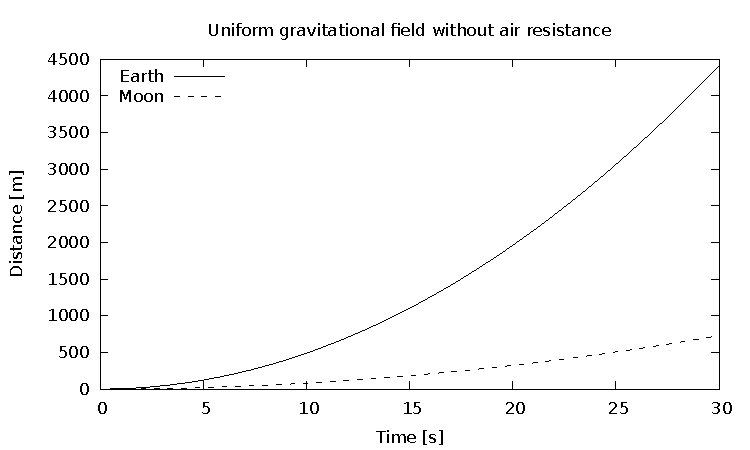
\includegraphics{gnuplot-bw}
% 	\caption{Černobílá varianta obrázku generovaného programem Gnuplot}\label{fig:gnuplot-bw}
% \end{figure}
% 
% \begin{figure}\centering
% 	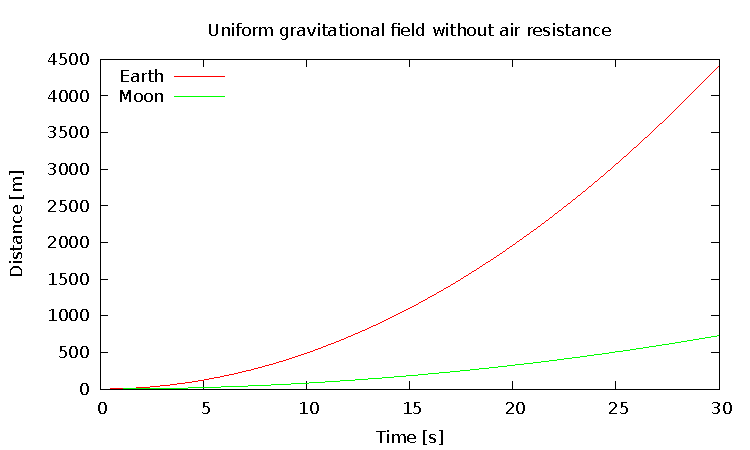
\includegraphics{gnuplot-col}
% 	\caption{Barevná varianta obrázku generovaného programem Gnuplot}\label{fig:gnuplot-col}
% \end{figure}
% 
% 
% \subsection{Tabulky}
% 
% Tabulky lze zadávat různě, např. v~prostředí \verb|tabular|, avšak pro jejich vkládání platí to samé, co pro obrázky -- použijte plovoucí prostředí, v~tomto případě \verb|table|. Například tabulka \ref{tab:matematika} byla vložena tímto způsobem.
% 
% \begin{table}\centering
% 	\caption[Příklad tabulky]{Zadávání matematiky}\label{tab:matematika}
% 	\begin{tabular}{|l|l|c|c|}\hline
% 		Typ		& Prostředí		& \LaTeX{}ovská zkratka	& \TeX{}ovská zkratka	\tabularnewline \hline \hline
% 		Text		& \verb|math|		& \verb|\(...\)|	& \verb|$...$|		\tabularnewline \hline
% 		Displayed	& \verb|displaymath|	& \verb|\[...\]|	& \verb|$$...$$|	\tabularnewline \hline
% 	\end{tabular}
% \end{table}
% 
% % % % % % % % % % % % % % % % % % % % % % % % % % % % 

\chapter{Obsah přiloženého CD}

object.rdfs

\begin{figure}
	\dirtree{%
		.1 readme.txt\DTcomment{stručný popis obsahu CD}.
		.1 exe\DTcomment{adresář se spustitelnou formou implementace}.
		.1 src.
		.2 impl\DTcomment{zdrojové kódy implementace}.
		.2 thesis\DTcomment{zdrojová forma práce ve formátu \LaTeX{}}.
		.1 text\DTcomment{text práce}.
		.2 thesis.pdf\DTcomment{text práce ve formátu PDF}.
		.2 thesis.ps\DTcomment{text práce ve formátu PS}.
	}
\end{figure}

\end{document}
